\documentclass[book.tex]{subfiles}
\begin{document}
id Software was funded during February 1991 by four people departing from SoftDisk: 

 \begin{figure}[H]
\centering  
\begin{tabularx}{\textwidth}{ X  X  X  }
  \toprule
  \textbf{Name} &  \textbf{Age} & \textbf{Occupation} \\
  \toprule 
   John Carmack & 22 &  Programming\\
   John Romero & 25 &  Programming\\
   Adrian Carmack & 22 &  Artist\\
   Tom Hall & 28 &  Creative Director\\
     \toprule
\end{tabularx}
\caption{id Software founding members.}\label{fig:Id Software team}
\end{figure}

Wolfenstein 3D was id first title but the team had already shipped no less than 13 games will working for their previous employer:
\begin{itemize}
  \item Dangerous Dave (1988)\footnote{Dangerous Dave is a solo project of John Romero predating Id's formation, but Id Software produced its first sequel and it is sometimes regarded as an early Id Software title. Later Dangerous Dave sequels were not made by Id, nor were later Catacomb titles.}
  \item Commander Keen
  \begin{itemize}
    \item Episode 1: Marooned on Mars (1990)
    \item Episode 2: The Earth Explodes (1991)
    \item Episode 3: Keen Must Die (1991)
    \item Keen Dreams (1991)
    \item Episode 4: Secret of the Oracle (1991)
    \item Episode 5: The Armageddon Machine (1991)
    \item Episode 6: Aliens Ate My Baby Sitter (1991)
  \end{itemize}
  
  \item Dangerous Dave in the Haunted Mansion (1991)
  \item Rescue Rover (1991)
  \item Rescue Rover 2 (1991)
  \item Shadow Knights (1991)
  \item Hovertank 3D (1991)
  \item Catacomb 3D: A New Dimension (1991)
\end{itemize}


Considering the magnitude and ambitions of the title, four more people were added to the team for a total of eight.\\
\note{TODO Ask team members if they know how old were Jay, Bobby, Robert and Jason}
 \begin{figure}[H]
\centering  
\begin{tabularx}{\textwidth}{ X  X  X  }
  \toprule
  \textbf{Name} &  \textbf{Age} & \textbf{Occupation} \\
  \toprule 
   Jay Wilbur & ?? &  Business\\
   Kevin Cloud\footnote{Jay and Kevin were recruited on April 1st, 1992 but were still given credits for participating to the game development.} & 27 &  Computer Artist\\
   Robert Prince & ?? &  Composer\\
   Jason Blochowiak & ?? &   Programming\\
     \toprule
\end{tabularx}
\caption{id Software hires.}\label{fig:Id Software hires}
\end{figure}

\begin{fancyquotes}
Jason was part of Id at the start, but we parted ways during Wolf development.
 \bigskip \\
\textbf{John Carmack - Programmer}
 \end{fancyquotes}\footnotetext{Jason still wrote part of the page manager and is credited for introducing John Carmack to Unix development
which ultimately led to the purchase of a Next Color ColorStation.}
 
\begin{figure}[H]
\centering
  \shadowbox{
      \fullimage{idTeam_team_pants.png}
  }  
\caption{The team as it appears in Spear of Destiny in a secret screen created by John Romero.}
\label{fig:id_team_1993}
\end{figure}
 
\begin{figure}[H]
\centering
  \shadowbox{
      \fullimage{id_team_with_pants.jpg}
  }  
\caption{They were in fact wearing pants.}
\label{fig:id_team_1993}
\end{figure}


Development took seven months (from November 1991 to May 1992) during which id Software was located in Madison, WI
\begin{figure}[H]
\centering
 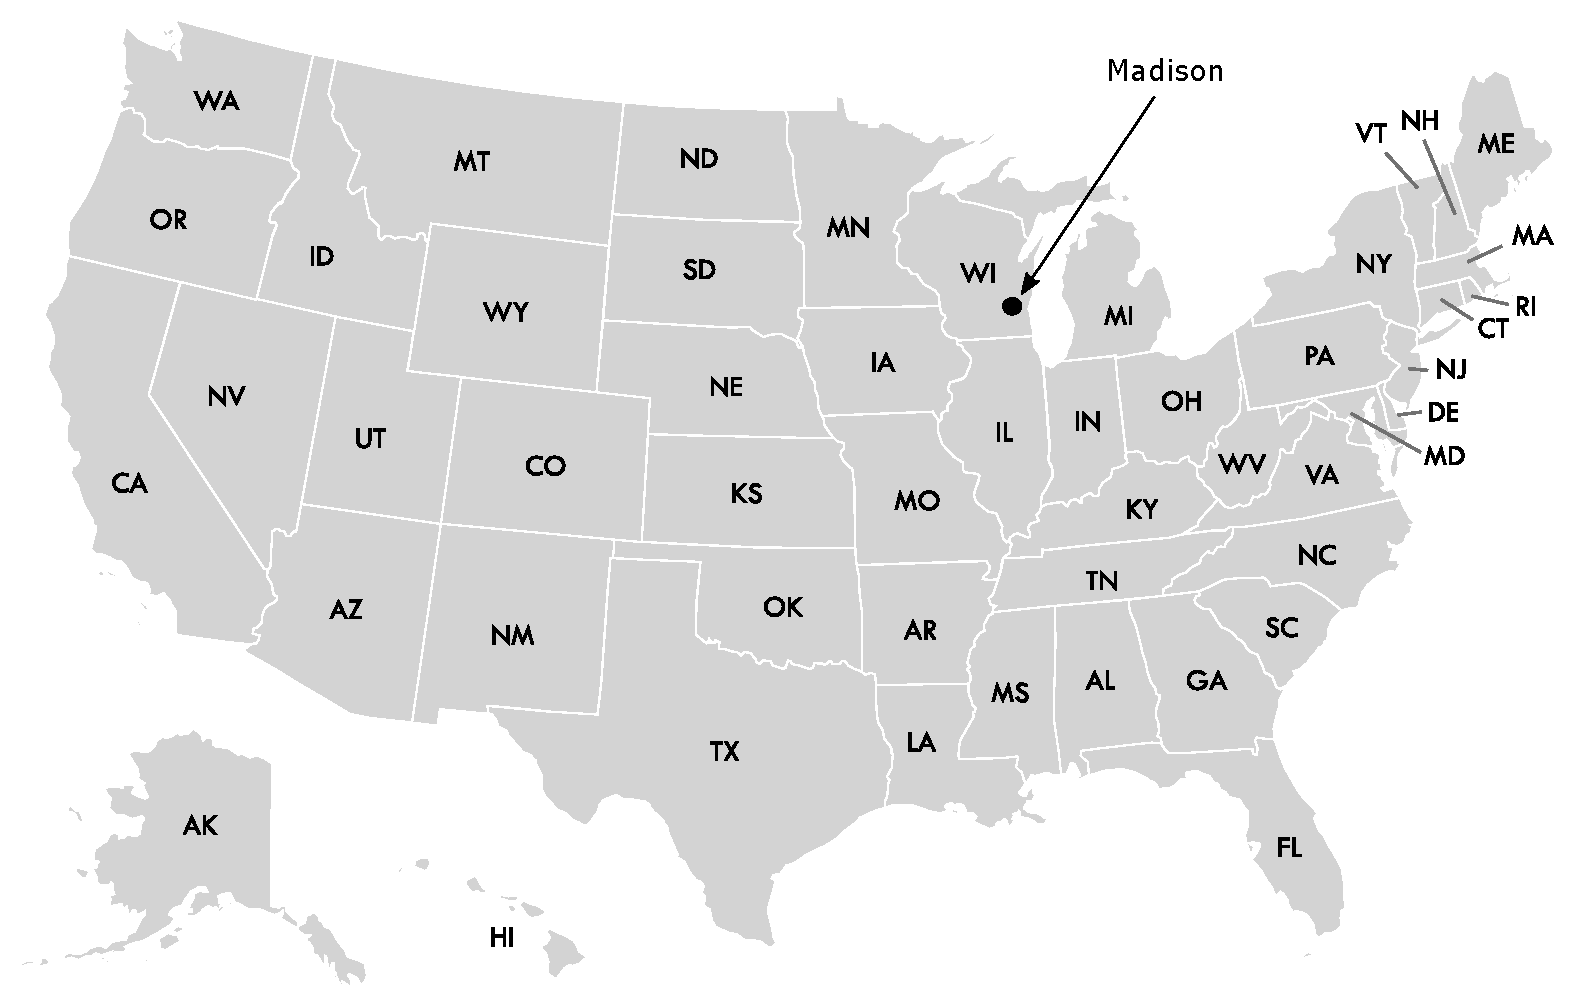
\includegraphics[width=\textwidth]{imgs/drawings/map/usa-id-software.eps}
 \end{figure}

\section{Office layout}
The organisation of the team was pretty much standard for a game studio of the early 90s: Four guys crammed in one room which allowed fast communication (and a lot of noise disturbance given John Romero and Tom Halls type of interaction). Notice on the upper floor, the SNES where countless games of F-Zero where played and the Donjon \& Dragons area extensively mentioned in "Masters of Doom" book. Not even having a team member with his apartment directly above the studio was out of the ordinary\footnote{90 Hours A Week And Loving It!}.\\
\par
The team was setup as follow\footnote{Since they played Dungeons \& Dragons a lot, the map is drawn D\&D style.}:
\par
\begin{figure}[H]
  \centering
  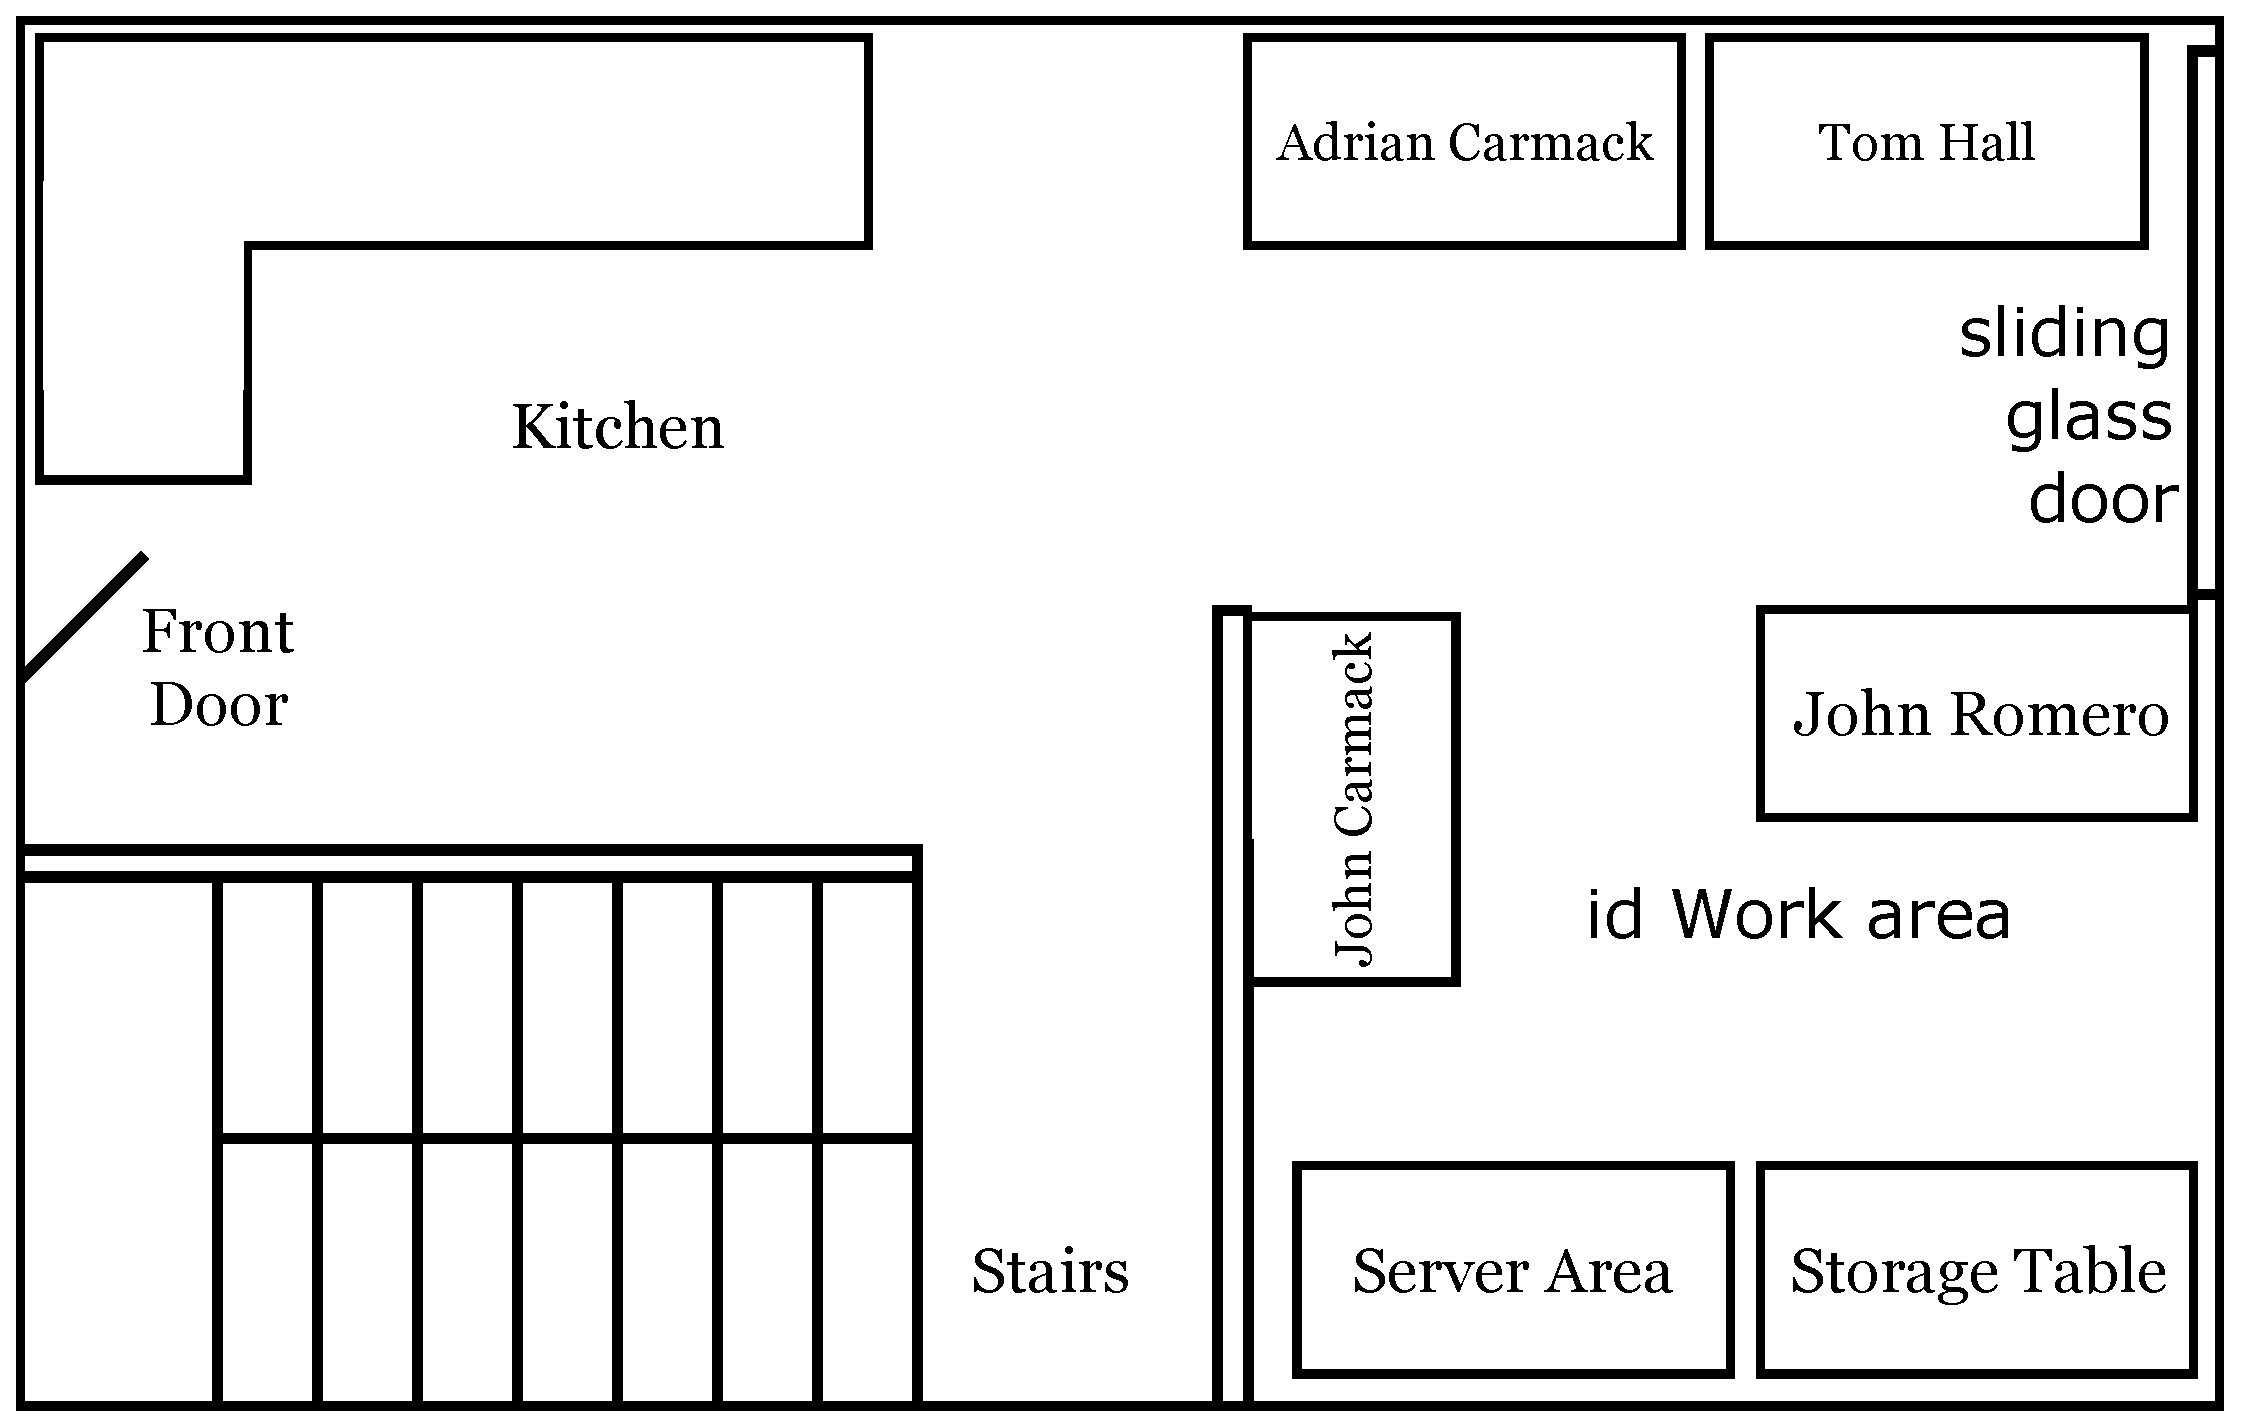
\includegraphics[width=\textwidth]{imgs/drawings/map/id-software-office-madison_bottom_floor.eps}
 %\caption{Office bottom floor.} 
\end{figure}
\par
\begin{figure}[H]
  \centering
  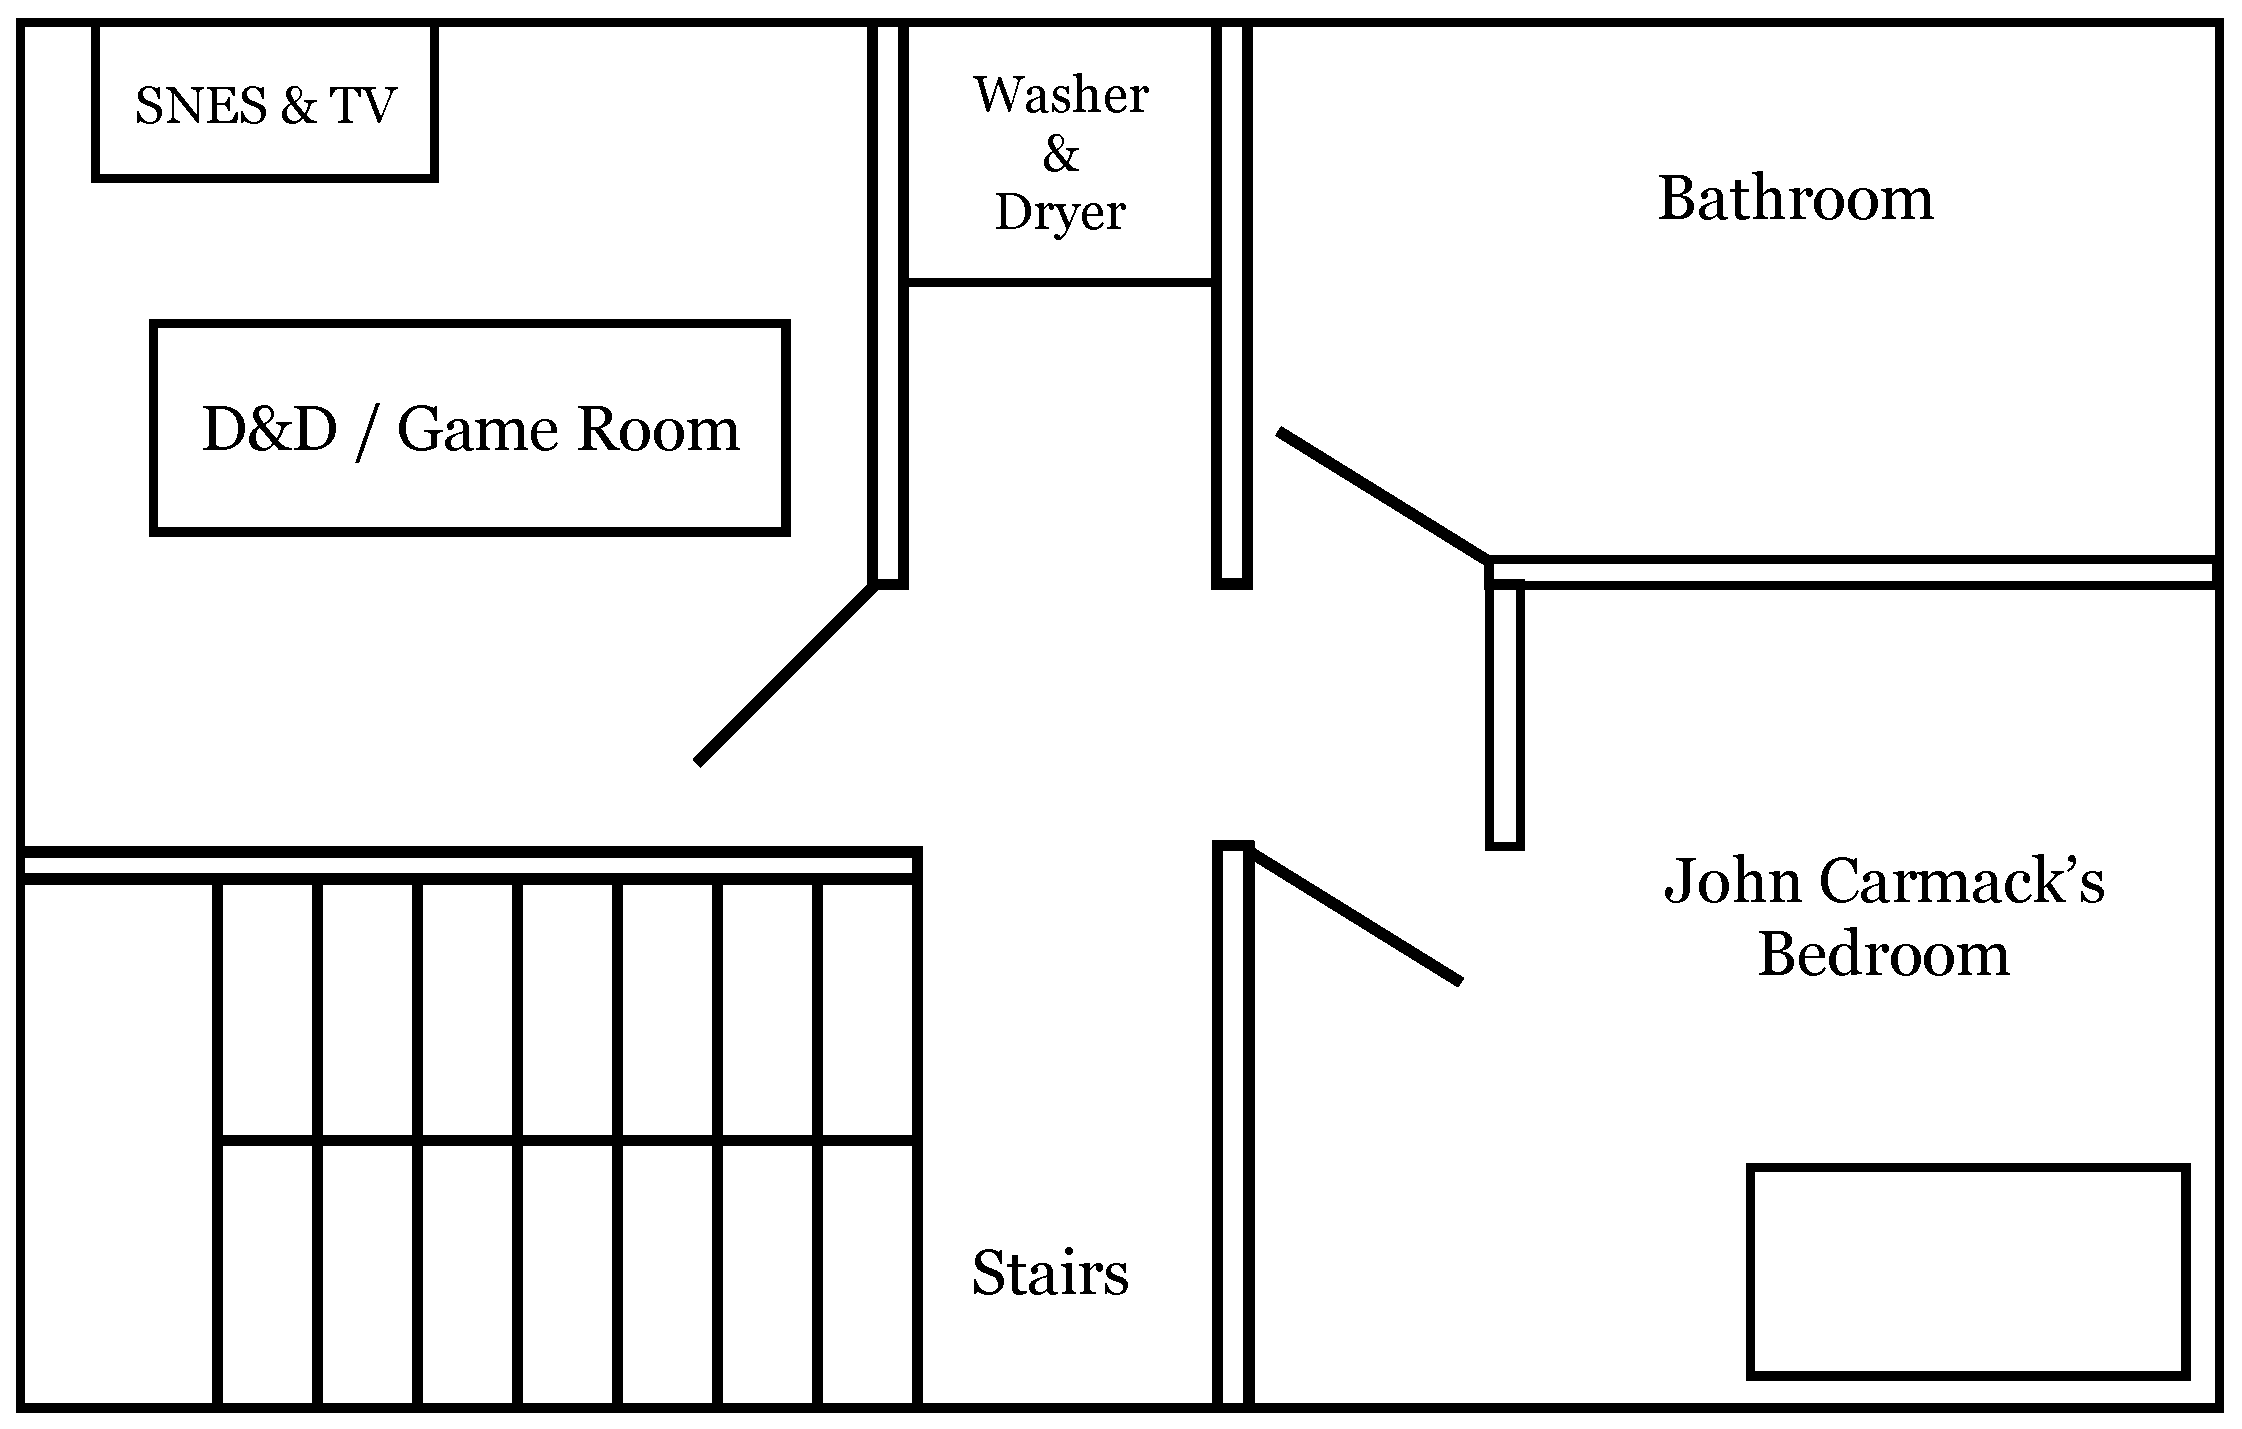
\includegraphics[width=\textwidth]{imgs/drawings/map/id-software-office-madison_top_floor.eps}
 %\caption{Office top floor.} 
\end{figure}
Everybody was working with an high end 386-DX 33Mhz. As for combining engine, tools and assets:\\

 \begin{fancyquotes}
We started with floppy data transfer, but we had a Novell network on coax Ethernet by the end. We didn't have a version control system.  Surprisingly, we went all the way to Quake 3 without one, then we started using Visual Source Safe.\\
 \\
\textbf{John Carmack - Programmer}
\end{fancyquotes}


























\section{Programming}



Development was done with Borland C++ 3.1 (however the language used was C): The editor uses VGA mode 3 offering a real estate of 80 characters wide and 25 characters tall.\\
\par
John Carmack took care of the runtime code. John Romero programmed many of the tools (TED map editor, packers, ...). Jason Blochowiak was contracted to write important subsystems of the game (Input manager, Page Manager, Sound Manager, User Manager).\\
\\
\begin{figure}[H]
\centering
  \shadowbox{
      \fullimage{development.png}
  }  
\caption{Bordland C++ 3.1 editor}
\end{figure}


To compensate for the tiny CRT display, some of the developers used two screens (an unusual thing at the time).\\

\begin{fancyquotes}
At that point, we wanted 21" monitors, but couldn't justify them.  I used a second mono monitor to allow Turbo Debugger 386 to keep the main screen in graphics mode while I stepped through the code.\\
 \\
\textbf{John Carmack - Programmer}
\end{fancyquotes}
\\
You may have noticed in the listing of VGA modes: 13h and 4h (figure~\ref{fig:vga_modes} on page~\pageref{fig:vga_modes})  don't have the same starting VRAM address. This allows for a neat trick where two graphic cards are plugged in the PC: One in monochrome text picking up data at 0xB000:0000 and the other one VGA picking up data at 0xA000:0000. This setup allows a developer to debug the game engine in real-time.\\
\begin{figure}[H]
\centering
  \shadowbox{
      \fullimage{wolf_screen1.png}
  }  
\caption{Monitor 1 with Bordland Turbo Debugger 386}
\label{fig:dm1}
\end{figure}

\begin{figure}[H]
\centering
  \shadowbox{
      \fullimage{wolf_screen2.png}
  }  
\caption{Monitor 2 running the game as normal}
\label{fig:dm1}
\end{figure}



 
 
 




\section{Graphics assets}
The graphic assets are divided as follow:
\begin{itemize}
\item 2D Menus items (pictures).
\item 3D Action phase items (walls and sprites).
\end{itemize}
Those were the work of Adrian Carmack\footnote{Kevin Cloud did a few textures and also worked on the design and layout of the Wofenstein 3D Hint book published eventually.}. All of the work was done with Deluxe Paint (from Electronic Arts) and saved in LBM files (Deluxe Paint format). 

\begin{figure}[H]
  \centering
 \fullimage{deluxe_paint.png}
 \caption{Deluxe Paint tool, used to draw all assets in the game.}
\end{figure}


\par
Since the VGA is palette based (colors a not specified via 24-bits RBG but by indices pointing to a 256 colors table) the creative process was difficult. The artist had first to make the key decision of what colors would go in the palette\footnote{Some games (such as Monkey island) used many palettes depending on the section of the game but id went for a simple solution: One palette for the whole game.} and then draw everything with only these colors.\\
\begin{figure}[H]
  \centering
\fullimage{palette.png}
 \caption{Wolfentein 3D palette: Everthing in the game is drawn using one of these 256 colors.}
\end{figure}
The Game palette with Horizontal from 0x00 to 0x0F, vertical from 0x00 to 0xF0. The blue gradient starts at 0xF0 and ends at 0xFE. 0xFF (represented in pink) is transparent color and always skipped during rendition.\\
\par

All assets were "hand" drawn with a mouse. Since the VGA would stretch the framebuffer when displaying it on the screen (from 320x200 to 320x240), Adrian had to be careful to draw at the same resolution as the game would run. To factor in these non-square pixels.\\
\par
\begin{fancyquotes}
We didn't have any scanning tools at the time.\\
\\
\textbf{John Carmack - Programmer}
\end{fancyquotes}
\\
















\section{Asset workflow}
As the graphic assets were generated by artists, a tool (IGRAB-ED) packed all the ILBMs files together in an archive and generated a C header file with asset IDs:. The engine references an asset directly by using these IDs.\\
\begin{figure}[H]
\centering
 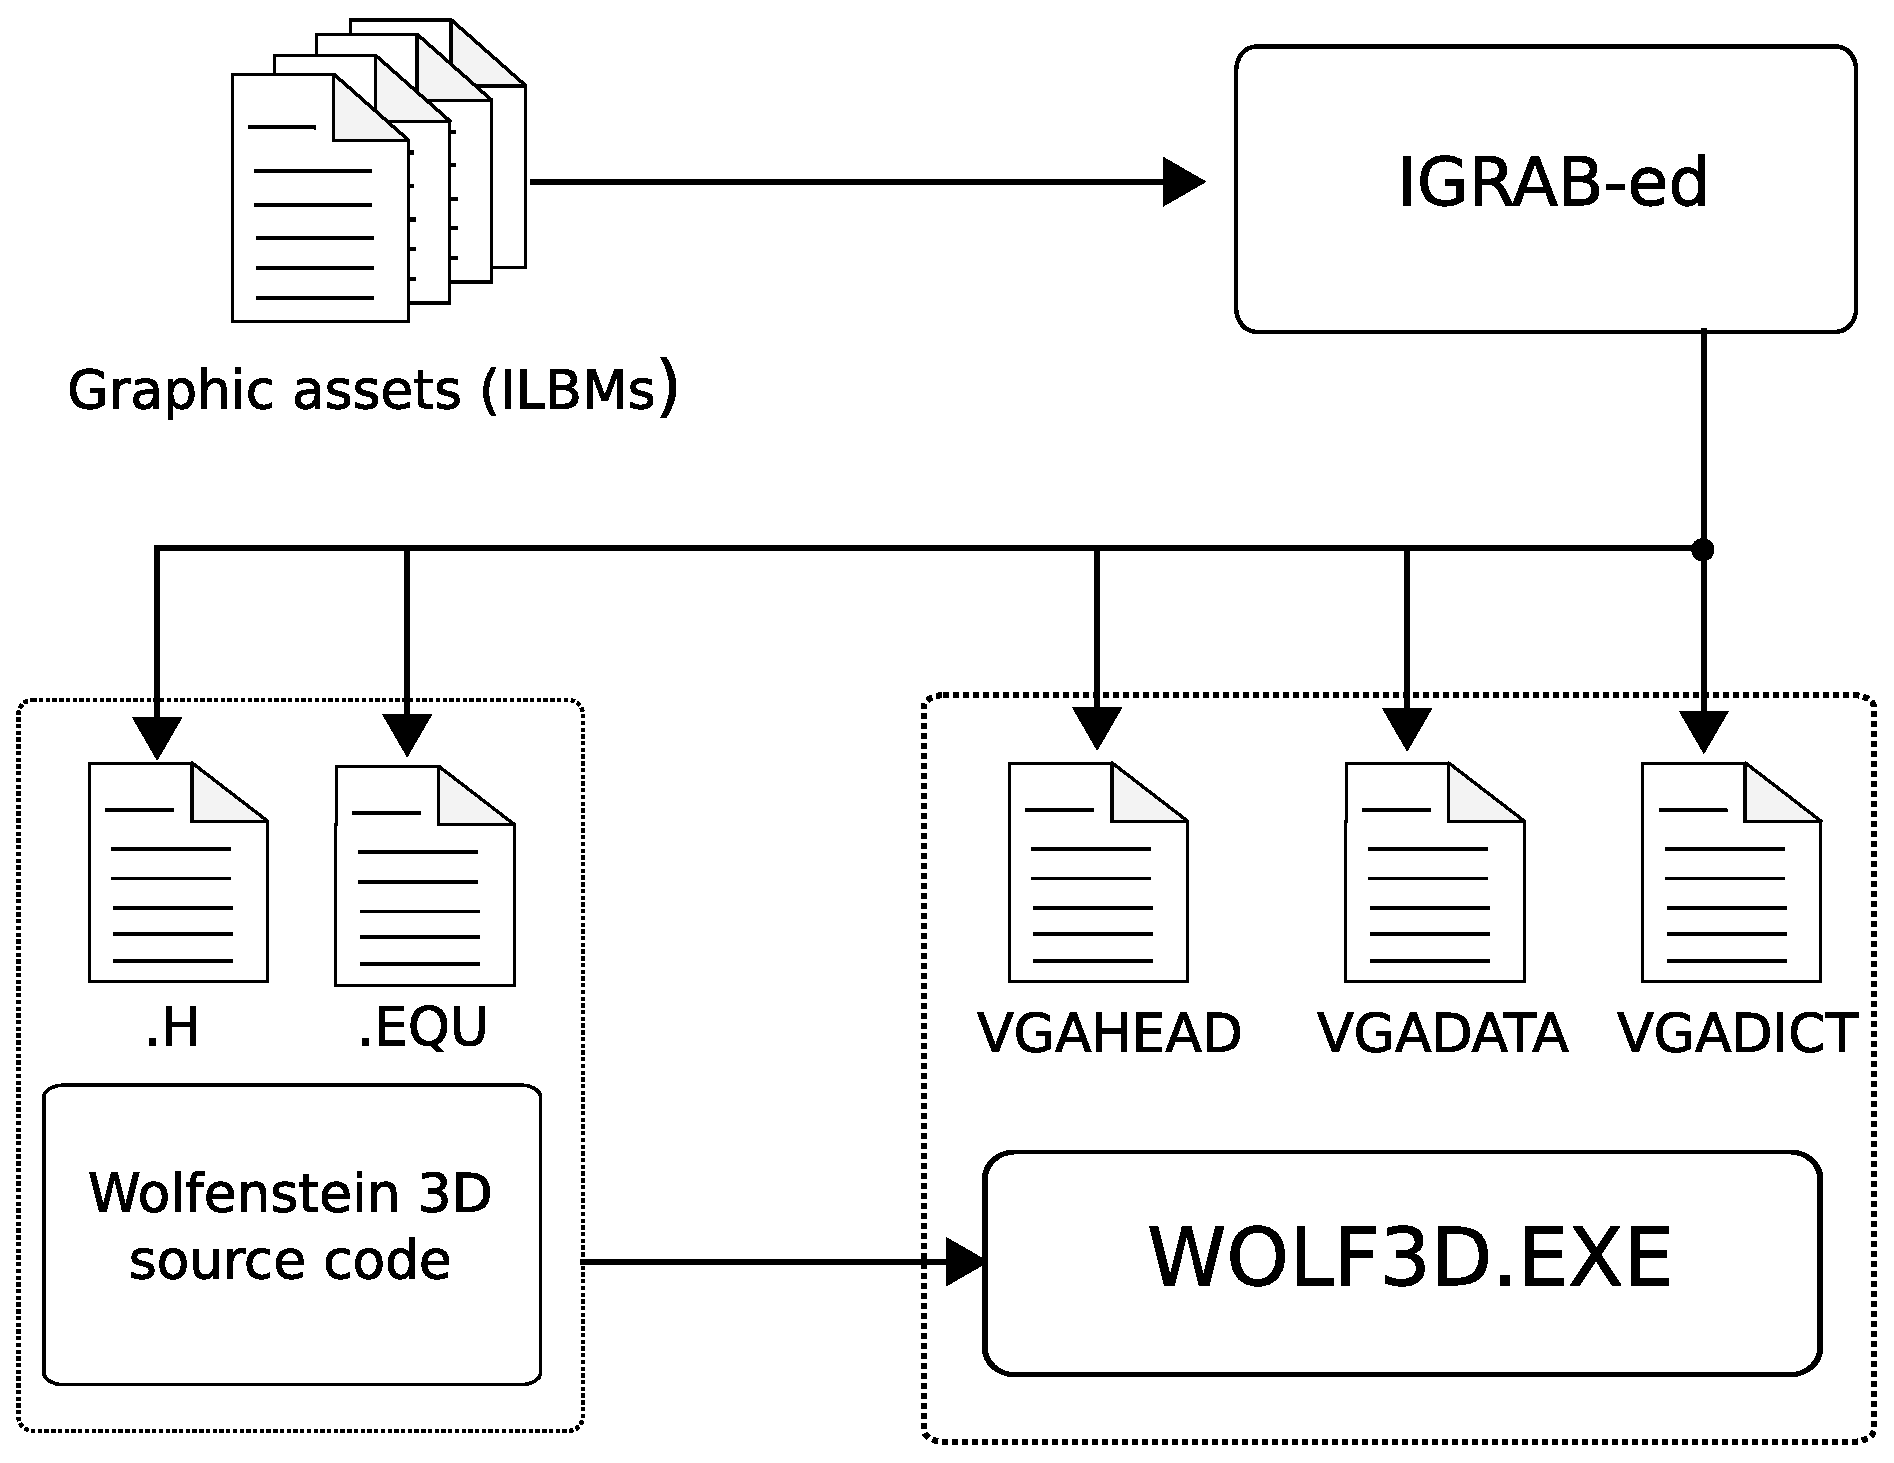
\includegraphics[width=\textwidth]{imgs/drawings/drawing_plain.eps}
 \caption{Assets creation} 
 \end{figure}

\begin{minipage}{\textwidth}
 \lstinputlisting[language=C]{code/assets_header.c}\par
 \end{minipage}
 
 In the engine, assets usage were "hardcoded" via the enum. Thanks to this indirection layer, the assets could be used in the engine yet nothing would have to be changed if the order of the assets changed in the \cw{VGA*} archives:\\
 \par
 \begin{minipage}{\textwidth}
 \lstinputlisting[language=C]{code/assets_usage.c}\par
 \end{minipage}
\par
\textbf{\underline{Trivia :}} This system let to issues when the source code was released: The \cw{.h} header files provided did not match the asset file from the shareware or early version of Wolfenstein 3D: The header released were from Spears of Destiny. You can see the kind of graphic mess this let to in the appendix "Let's compile like it is 1994".\\




\begin{minipage}{0.7\textwidth}
\bu{Trivia :} "The Official Hint Manual for Wolfesnteind 3D" published in 1992 contains many drawing from Tom Hall and shows many behind the scene sketches made by Tom Halls and pixel arted by the graphic team.\\
\par
 \begin{fancyquotes}
When Id's Creative Director, Tom Hall gets an idea for a screen, he provides a sketches for Adrian Carmack. Below are some of Tom's early design for the title screen. The third sketch was chosen.\\
\end{fancyquotes}
\end{minipage}
\begin{minipage}{0.3\textwidth}
\begin{flushright}
\fullimage{hint_manual_cover.png}
\end{flushright}
\end{minipage}

\noindent
   \begin{figure}[H]
\centering
 \fullimage{sprites/tom_hall_sketch_intro_screen_genesis.png}
 \end{figure}
 \par
   \begin{figure}[H]
\centering
 \scaledimage{.7}{sprites/woldf3d.png}
\end{figure} 

\footnotetext{The manual was entirely designed on a NeXT ColorStation. It was the only usage of NeXT for Wolfenstein 3D (they purchased it in december 1991).}


\begin{figure}[H]
\centering    
     \fullimage{sprites/tom_hall_sketch_adolf.png}
   \end{figure}

     \begin{figure}[H]
\centering
     \fullimage{sprites/tom_hall_sketch_dr_schabbs.png}
   \end{figure}
 
  \begin{figure}[H]
\centering
 \scaledimage{0.8}{sprites/tom_hall_sketch_gretel.png}\\
 \end{figure}








      \begin{minipage}{.48\textwidth}
     \fullimage{sprites/tom_hall_sketch_officer.png}
  \end{minipage}
      \begin{minipage}{.48\textwidth}
     \fullimage{sprites/fettgesic.png}
  \end{minipage}

       \begin{minipage}{.48\textwidth}
     \fullimage{sprites/tom_hall_sketch_officer2.png}
  \end{minipage}
      \begin{minipage}{.48\textwidth}
     \fullimage{sprites/giftmacher.png}
  \end{minipage}\\

\par 
The hint manual also contains several photos of the team back in the days. Go check it out!













\section{Maps}
Maps were created using the in-house editor called TED5 which is short for Tile EDitor. TED was not create specially for wolf: It was actually created way back during Commander Keen serie (yes: a platform scroller) and improved over the years. TED does not stand-alone. In order to start it needs an asset archive and the header associated (as described in the graphic asset workflow). This way texture ids are directely encoded in the map.\\

 \begin{figure}[H]
\centering
 \fullimage{ted5_scrolling_map.png}
 \caption{TED used for Commander Keen - side scroller} 
 \end{figure}


\begin{figure}[H]
\centering
 \fullimage{TED.png}
 \caption{TED used for top view level design} 
 \end{figure}

Reusing TED was a double win: It saved tool development time and since all team members had been using it for years, they were all proficient with it: No need to learn it. TED5 allowed id to make many levels within a small amount of time:\\
\par

 \begin{fancyquotes}
After talking with Romero and Tom, Scott learned that it was taking the group only about one day to make a level of the game. Ka-chung! Dollar signs! Instead of just three episodes, why not have six? Scott said, "If you can do thirty more levels, it would only take you fifteen days. And we could have it where people could buy the first trilogy for thirty-five dollars or get all six for fifty dollars, or if people buy the first episode and later want the second episodes it will be twenty dollars. So there’s a reason to get them all!" After some consideration, id agreed.\\
\\
 \textbf{- Masters of Doom}
 \end{fancyquotes}\\

\bu{Trivia :} When the engine was licensed to Apogee for Rise of The Triad, TED5 was also used. Tom Halls wrote about it and you can find his comment in the Appendix section.\\
\par
Everybody worked a little bit on the map but those were mostly the work of John Romero and Tom Hall.\\
\par
 \textbf{\underline{Trivia :}} The source code of TED5 was released several years later. Inspecting the source was a mysterious \codeword{\_TOM.PIC}. Converted to PNG it looks as follow:\\
\begin{figure}[H]
\centering
 
\includegraphics[width=\textwidth]{imgs/drawings/_tom.pdf}
 \caption{Not so politically correct caricature.} 
 \end{figure}
The explanation was provided later by John Romero:\\
 \begin{fancyquotes}
   "Hahahaha! Wow, I forgot all about that picture. I can't believe it's 
in the TED5 source files! It's basically a pic that Adrian drew of Tom 
getting Adrian's dick blasted into his face with Adrian saying "Sorry!". 
It's because Tom and Adrian used to share a worktable together and Tom 
would always bump the table while Adrian was drawing graphics with the 
mouse and Tom would say, "Sorry!" That picture never appears in Ted5 
anywhere.\\
   \\
\textbf{John Romero - Programmer}
 \end{fancyquotes}\\











\section{Audio}

\subsection{Sounds}
As mentioned in the hardware section, the audio hardware was highly fragmented. id decided to support four sound cards and the default PC speaker. Which meant generating assets multiple times for each hardware and pack them together with an in-house too called MUSE into AUDIOT archives (an id software proprietary format):\\
\begin{figure}[H]
\centering
 \fullimage{muse.png}
 \end{figure}
 \par
\note{Sound production pipeline. How were voice recorded ? Where are Mein Leben (My life) and Achtung(Attention) coming from?}


\subsection{Music}
All composition was done by Robert Prince:\\
\par
 \begin{fancyquotes}
In the early days of the OPL soundcards, the "gold standard" sequencing software was Sequencer Plus Gold ("SPG") by Voyetra. The reason for this was it had an OPL instrument/instrument bank editor.\\
\par
To rough out compositions, I used Cakewalk ("CW"). I had been using it for several years already and had it all set up to use the analog boxes for sound output. Having "real" sounds from those boxes helped me visualize (audiolize?) what I wanted musically. I would save the CW files in *.mid format and load them into SPG to create the OPL instrument for each track. I built different instrument banks for the different genres of music.

\textbf{Bobby Prince - Composer}
 \end{fancyquotes}\\

\begin{figure}[H]
\centering
  \shadowbox{
      \fullimage{music_editor.png}
  }  
\caption{Sequencer Plus Gold ("SPG") by Voyetra}
\end{figure}



\bu{Trivia :} In Episode 3 the music playing features a hidden Morse coded message. "To Big Bad Wolf. De Little Red Riding Hood. Eliminate Hitler. Imperative. Complete mission within 24 hours. Out.". The end boss of this episode indeed is Hitler in a Mech suit (see hint drawing).




























\section{Distribution}
The game distribution model was shareware: The game engine along with one single episode were given for free and encouraged to be copied and distributed to a maximum number of peoples. To get the five other episodes, player had to mail \$50 by mail.\\
\par
\begin{figure}[H]
\centering
 \fullimage{shareware.png}
 \caption{User exits the game back to DOS prompt: A message shows how to get the full version.}
 \end{figure}

\end{document}
\par
It was therefore paramount to make the game easy to copy. In 1991, Internet was still in its infancy and the best medium was the  3\nicefrac{1}{2}-inch floppy. A particular attention to the size of the package was given. All assets combined accounted for 1,204KB but everything was compressed to 645KB (a 3\nicefrac{1}{2}-inch floppy can store 720KB). The full six episodes fit on two disks. Spears of Destiny would fit on three disks.
The game shipped as follow:\\
\par
 \begin{figure}[H]
\centering
 \fullimage{result.png}
 \caption{Tile EDitor screen} 
  \end{figure}
  \par
 The files can be divided in five parts:
 \begin{itemize}
 \item WOLF3D.EXE: The Game engine.
 \item VSWAP.WL1: Contains all the assets (sprites, textures, digitized sound) needed during 3D action phases.
 \item Music files used during both 3D and 2D phases:
     \begin{itemize}
     \item AUDIOHED.WL1 : Index to payload in \cw{AUDIOT} file.
     \item AUDIOT.WL1: Uncompressed audio data. 
     \end{itemize}
\item Maps:
     \begin{itemize}
     \item MAPHEAD.WL1 : Index into \cw{GAMEMAPS} file.
      \item GAMEMAPS.WL1 : Compressed Map payloads.
      \end{itemize}
\item Pictures used during 2D menus phase:
    \begin{itemize} 
    \item VGAHEAD.WL1 : Index into \cw{VGAGRAPH} file.
    \item VGADICT.WL1 : Huffman-tree to decompress each the picture.
    \item VGAGRAPH.WL1 : Compressed pics lumped together.
     \end{itemize}
\end{itemize}
 \par

\textbf{\underline{Trivia :}} The file extension did have a meaning: 
\begin{itemize}
\item WL1: Shareware.
\item WL3: Early three-episode full version (never released).
\item WL6: Six-episode full version.
\item WJ1: Japanese shareware.
\item WJ6: Japanese full version.
\item SOD: Spear of Destiny.
\end{itemize}
 
\textbf{\underline{Trivia :}}The engine is very tiny and only occupy 94KB. But with 64KB dedicated to the Signon screen and 768B for the palette, the engine is in fact only 29KB of instructions.\\